
\begin{frame}
 \frametitle{Quality control: Overview}

Quality control for software:
\begin{itemize}
  \item Known: Software errors occur in practice.
  \item Goal: Prevent errors \textbf{at least} in live software.
\end{itemize}
Options?
 \pause
\begin{itemize}
  \item Code Review
   \begin{itemize}
    \item four-eyes principle
    \item Team Review, if applicable via pair programming
   \end{itemize} \pause
  \item Tests
   \begin{itemize}
    \item Manually
    \item Automatically
   \end{itemize} \pause
  \item Formal methods
   \begin{itemize}
    \item Formal verification
    \item Proofs of Program Correctness 
   \end{itemize}
\end{itemize}
\end{frame}

%%%%%%%%%%%%%%%%%%%%%%%%%%%%%%%%%

\begin{frame}
\frametitle{Things we do not want: Bugs}
%\framesubtitle{\citep{Binder1999}}
  \begin{center}
  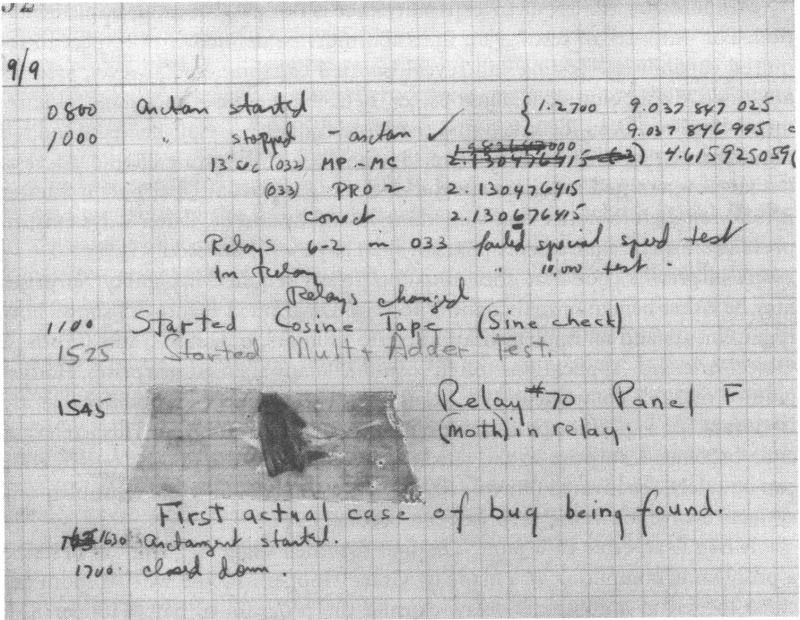
\includegraphics[width=.85\textwidth]{images/Qualitaetssicherung/abbildungen/Bug}
  \end{center}

\end{frame}

%%%%%%%%%%%%%%%%%%%%%%%%%%%%%%%%%

\section{Validation \& Verification}

%%%%%%%%%%%%%%%%%%%%%%%%%%%%%%%%%

\begin{frame}
\frametitle{Validation and verification of software}
\begin{itemize}
  \item Validation and verification of the implemented software system:%\citep{Boehm1984,FisherVV2007}:
    \begin{itemize}
      \item "`Do we build the system right?"' (Verification)\\
            Check  that the system meets the requirements
      \item "`Do we build the right system?"' (Validation)\\
            Check whether the \emph{actual} (user) requirements have been realized.
    \end{itemize}
  \item Validation can be supported e.g. by prototyping (see LE \ref{sec:Process_Models})
  \item Occasionally these terms are also used differently:
    \begin{itemize}
      \item e.g. verification for formal proofs and validation for \emph{running}.
    \end{itemize}
\end{itemize}
\end{frame}

%%%%%%%%%%%%%%%%%%%%%%%%%%%%%%%%%

\begin{frame}\frametitle{Validation and Verification: Roles}
\begin{center}
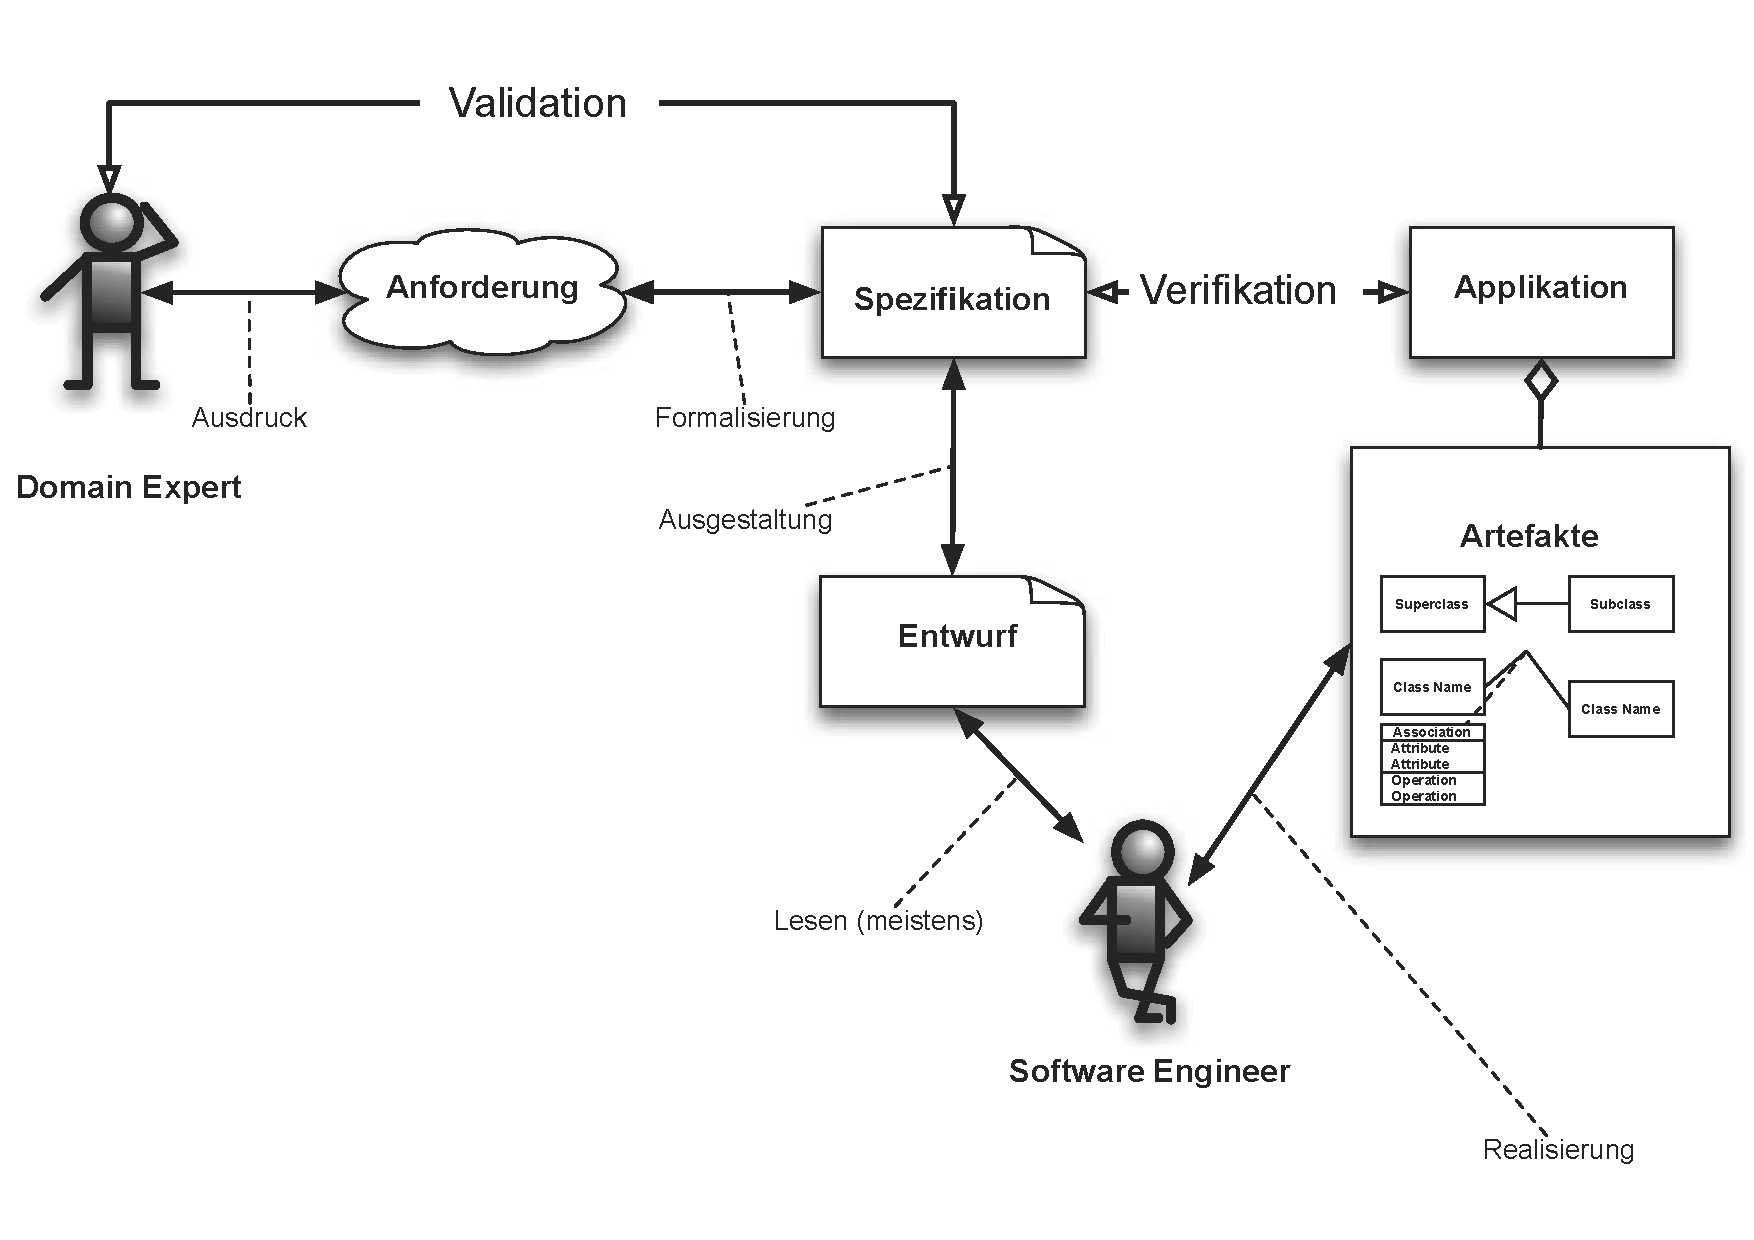
\includegraphics[width=\textwidth]{images/Qualitaetssicherung/abbildungen/ValidationVerifikation}
\end{center}
\end{frame}

%%%%%%%%%%%%%%%%%%%%%%%%%%%%%%%%%

\begin{frame}
\frametitle{Verification Objectives}
\begin{itemize}
  \item Proof of the correct functioning of all functions of a system in relation to a given specification
    \begin{itemize}
      \item Identify errors
      \item Absence of errors
    \end{itemize}
  \item The verification process itself must also be verified: 
    \begin{itemize}
      \item Are the test conditions correct?
      \item Is a formal proof correct? 
    \end{itemize}
  \item Technical (non-functional) requirements must also be checked:
    \begin{itemize}
      \item Efficiency, portability, modifiability, etc.
    \end{itemize}
  \item The result is not always simply \emph{correct} or \emph{incorrect}.
    \begin{itemize}
      \item Reliability requirements and subjectivity require more fine-grained metrics,\\
      e.g. \emph{good enough} or 99\% availability.
    \end{itemize}
\end{itemize}
\end{frame}



%%%%%%%%%%%%%%%%%%%%%%%%%%%%%%%%%

\begin{frame}
\frametitle{Classification of verification techniques}

\begin{block}{Symbolic Execution}
The behavior of the system is tested with respect to the expected behavior.
\begin{itemize}
  \item Structure-oriented methods\\
        white-box, with knowledge of the implementation 
  \item Function-oriented methods\\
        black-box, without knowledge of the implementation
\end{itemize}
\end{block}
%Verification https://www.researchgate.net/figure/Classification-of-verification-techniques_fig3_36374045
%veritesting https://dl.acm.org/doi/abs/10.1145/2568225.2568293
%white-box fuzz testing http://pxzhang.cn/paper/concolic_testing/FuzzTesting.pdf
%concolic testing https://dl.acm.org/doi/abs/10.1145/1065010.1065036
 
\vspace{1ex}
\begin{block}{Static Analysis}
The behavior of a system is analyzed to derive whether the behavior is correct.
\begin{itemize}
  \item Static proofs of correctness
  \item Reviews, inspections, walkthroughs, etc.
\end{itemize}
\end{block}
\end{frame}

%%%%%%%%%%%%%%%%%%%%%%%%%%%%%%%%%
\subsection{Testing}

\begin{frame}
\frametitle{Testing for verification}
\begin{description}[Integration test]
  \item[Unit-Test]
  Single functions / components are tested.
  \item[Integration test]
  Interdependent components are tested together.\\
            Focus on interface testing.\\
        Components are integrated into subsystems and tested together.
  \item[System test]
  Test of the complete system.
\end{description}  
\begin{block}{Objective of a test planning}
Select test cases in such a way that the probability of finding errors or ruling them out is high.
\end{block}
\end{frame}

%%%%%%%%%%%%%%%%%%%%%%%%%%%%%%%%%

\begin{frame}
\frametitle{The V-Model}
\framesubtitle{Use especially by military and governmental authorities.}
\begin{center}
\pgfimage[width=\textwidth]{images/Qualitaetssicherung/abbildungen/VModel}
\end{center}
Verification and validation of the sub-products are essential components of the V-Model.
\end{frame}
%https://www.researchgate.net/figure/V-model-for-software-development_fig2_36374045

%%%%%%%%%%%%%%%%%%%%%%%%%%%%%%%%%

\begin{frame}
\frametitle{Problems in software testing}
\begin{itemize}
  \item Test cases often describe the behavior more detailed than the specification: 
    \begin{itemize}
      \item[$\rightarrow$] Develop test cases before implementation
    \end{itemize}
  \item Basic problem: \\
        ``Program testing can be used to show the presence of bugs, but never to show their absence.'' %\citep{Dijkstra72}
  \item Questions to answer:
   \begin{itemize}
  	\item How to determine suitable test cases and test plans? 
    \item How to check the correctness of the test implementation? 
    \item Who is the tests authority? 
   \end{itemize}
\end{itemize}
\end{frame}

%%%%%%%%%%%%%%%%%%%%%%%%%%%%%%%%%

%\begin{frame}
%\frametitle{The test process}
%\framesubtitle{\citep{Sommerville2018}}
  %\begin{center}
  %\includegraphics[width=1.05\textwidth]{images/Qualitaetssicherung/abbildungen/TestProcess}
  %\end{center}
%This represents a possible test process oriented to the V-Model.
%\end{frame}

%%%%%%%%%%%%%%%%%%%%%%%%%%%%%%%%%

\begin{frame}
\frametitle{Challenges of the steps in the test process}
    \begin{itemize}
    \item Identification of test scenarios (use cases)
         \begin{itemize}\item What is to be tested?
         \end{itemize} 
    \item Establishment of concrete test scenarios
          \begin{itemize}
           \item How is the test candidate executed?
           \item What is the correct behavior?
          \end{itemize} 
    \item Formalization of tests 
         \begin{itemize}\item How is the test specified? 
         \end{itemize} 
    \item Carrying out tests 
         \begin{itemize}\item Automation!
         \end{itemize} 
    \item Maintenance of tests
         \begin{itemize}\item Synchronized with the changes in the business software, the tests must (mostly) be adapted and modified.
         \end{itemize} 
    \end{itemize}
\end{frame}

%%%%%%%%%%%%%%%%%%%%%%%%%%%%%%%%%

\begin{frame}
\frametitle{Objectives for software testing}
\begin{itemize}
  \item It must be clear what results are expected when testing.
  \item Use of \emph{systematic} methods:
    \begin{itemize}
      \item Selection of test cases if possible not (only) intuitive or random.
    \end{itemize}
  \item The results should be fully reproducible. 
    \begin{itemize}
      \item This is a major problem especially when testing parallel programs.
    \end{itemize}
  \item Errors should not only be detected, but also localized and fixed. %\citep{Rohr2007}.
    \begin{itemize}
      \item \glq Known bugs\grq\ are not a sign of high quality software.
    \end{itemize}       
  \item Quality requirements must be checked with the highest accuracy possible.
\end{itemize}
\end{frame}

%%%%%%%%%%%%%%%%%%%%%%%%%%%%%%%%%

\begin{frame}
\frametitle{Pragmatic view on testing}
\begin{itemize}
    \item Testing allows conclusions about the quality of a software system 
    \item Quantitative metrics support conclusions 
         \begin{itemize}\item Test coverage etc. 
         \end{itemize} 
    \item Automated regression tests provide protection against side effects of modifications 
		\begin{itemize}
			\item A regression test is the repetition of test cases to ensure that modifications in already tested parts of the software do not cause new errors (``regressions''). 
		\end{itemize}
\end{itemize}
\end{frame}

%%%%%%%%%%%%%%%%%%%%%%%%%%%%%%%%%

\begin{frame}
\frametitle{Black-Box vs. White-Box Testing}
  \begin{center}
  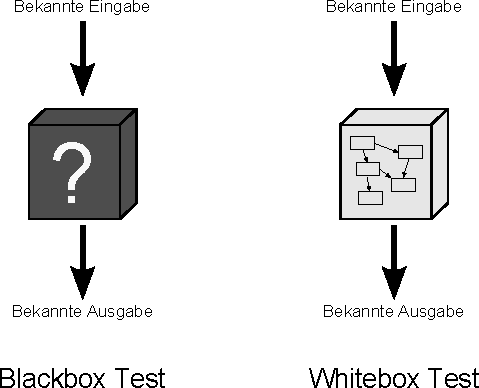
\includegraphics[width=.8\textwidth]{images/Qualitaetssicherung/abbildungen/BlackBoxAndWhiteBoxTesting}
  \end{center}
\end{frame}

